\documentclass[a4paper, 12pt, oneside]{Thesis}  

\usepackage[T1]{fontenc}
\usepackage[utf8]{inputenc} 


\usepackage{amsthm}
\usepackage{graphicx}
\usepackage{caption}
\usepackage{lineno}
\usepackage{makeidx}
\usepackage{color}
\usepackage{rotating}
\usepackage{longtable}
\usepackage{lscape,epsfig}
\usepackage{eurosym}
\usepackage{natbib}

\hypersetup{
colorlinks,
citecolor=blue,
filecolor=black,
linkcolor=red,
urlcolor=blue
}

\setcounter{MaxMatrixCols}{10}

\captionsetup{position=above,
              labelsep=colon,
              labelfont={normalsize,bf},
              textfont={normalsize},
              skip=0.75cm,
              justification=justified,
              margin=1cm}
\vfuzz3pt
\hfuzz8pt
\widowpenalty=20000 \clubpenalty=20000

\addtolength{\oddsidemargin}{0cm}
\addtolength{\evensidemargin}{0cm}
\addtolength{\topmargin}{-0.5cm}
\addtolength{\textwidth}{0cm}
\addtolength{\textheight}{1.5cm}
\renewcommand{\baselinestretch}{1.5} 

%\bibliographystyle{econometrica}
%\bibliographystyle{natbib}


\begin{document}
\frontmatter	  % Begin Roman style (i, ii, iii, iv...) page numbering

% Set up the Title Page
\title  {TITEL}
\authors  {\texorpdfstring
            {\href{EMAIL@unil.ch}{NAME}}
            {NAME}
            }
\addresses  {\groupname\\\univname}  % Do not change this here, instead these must be set in the "Thesis.cls" file, please look through it instead
%\addresses  {\groupname\\\deptname\\\univname}
\date       {January 1, 2020\\
\vspace*{3cm}

\includegraphics[trim= 0.1cm 0cm 0cm 0cm,clip,scale=1 ]{logoHEC.jpg}
\hfill

\includegraphics[trim= 0.1cm 0cm 0cm 0cm,clip,scale=1 ]{logoUNIL.jpg}
}


\maketitle
%% ----------------------------------------------------------------

\setstretch{1.5}  % It is better to have smaller font and larger line spacing than the other way round

% Define the page headers using the FancyHdr package and set up for one-sided printing
\fancyhead{}  % Clears all page headers and footers
\rhead{\thepage}  % Sets the right side header to show the page number
\lhead{}  % Clears the left side page header

\pagestyle{fancy}  % Finally, use the "fancy" page style to implement the FancyHdr headers

%% ----------------------------------------------------------------
% Declaration Page required for the Thesis, your institution may give you a different text to place here
\Declaration{

\addtocontents{toc}{\vspace{1em}}  % Add a gap in the Contents, for aesthetics

I, NAME, declare that this thesis titled, `TITLE' and the work presented in it are my own. I confirm that:

\begin{itemize} 
\item[\tiny{$\blacksquare$}] This work was done wholly or mainly while I worked for XYZ.
 
\item[\tiny{$\blacksquare$}] Where I have consulted the published work of others, this is always clearly attributed.
 
\item[\tiny{$\blacksquare$}] Where I have quoted from the work of others, the source is always given. With the exception of such quotations, this thesis is entirely my own work.
 
\item[\tiny{$\blacksquare$}] I have acknowledged all main sources of help.
 
\item[\tiny{$\blacksquare$}] Where the thesis is based on work done by myself jointly with others, I have made clear exactly what was done by others and what I have contributed myself.
\\
\end{itemize}
 
 
Signed:\\
\rule[1em]{25em}{0.5pt}  % This prints a line for the signature
 
Date:\\
\rule[1em]{25em}{0.5pt}  % This prints a line to write the date
}
\clearpage  % Declaration ended, now start a new page

%% ----------------------------------------------------------------
% The Abstract Page

\addtotoc{Abstract}  % Add the "Abstract" page entry to the Contents
\abstract{
\addtocontents{toc}{\vspace{1em}}  % Add a gap in the Contents, for aesthetics

Thesis abstract written here. Max $\frac{1}{2}$ of a page, both in Englisch \& French.\ldots

}

\clearpage  % Abstract ended, start a new page

%% ----------------------------------------------------------------

\setstretch{1.5}  % Reset the line-spacing to 1.5 for body text (if it has changed)

% The Acknowledgements page, for thanking everyone

\acknowledgements{
\addtocontents{toc}{\vspace{1em}}  % Add a gap in the Contents, for aesthetics

The acknowledgements and the people to thank go here, don't forget to include your project advisor.

}
\clearpage  % End of the Acknowledgements
%% ----------------------------------------------------------------
% The Executive Summary page

\executivesummary{
\addtocontents{toc}{\vspace{1em}}  % Add a gap in the Contents, for aesthetics

The executive summary should go here. Write about 2 pages\ldots

}
\clearpage  % End of the Executive Summary

%% ----------------------------------------------------------------

\pagestyle{fancy}  %The page style headers have been "empty" all this time, now use the "fancy" headers as defined before to bring them back




%% ----------------------------------------------------------------
\mainmatter	  % Begin normal, numeric (1,2,3...) page numbering
\pagestyle{fancy}  % Return the page headers back to the "fancy" style

% Include the chapters of the thesis, as separate files
% Just uncomment the lines as you write the chapters

% Chapter 1

\chapter{Introduction} % Write in your own chapter title
\label{Chapter1}
\lhead{Chapter 1. \emph{Introduction}} % Write in your own chapter title to set the page header

\section{Introduction}

TEXT %

%\input{./Chapters/Chapter2} %
What follows is a reference:
\cite{merton1973theory}


%% ----------------------------------------------------------------
\label{Bibliography}
%%%%%%%%%%%%%%%%%%%%%%%%%%%%%%%%%%%%%%%%%%%%%%%%%%%%%
\bibliography{bibliography}
%%%%%%%%%%%%%%%%%%%%%%%%%%%%%%%%%%%%%%%%%%%%%%%%%%%%%
\clearpage\newpage
%% ----------------------------------------------------------------
% here come the tables
\lhead{\emph{Tables}}  % Change the left side page header to "Bibliography"
\begin{center}
{\Huge Tables}
\end{center}

\begin{center}
{ 
\begin{tabular}{c|cc|cc}
& \multicolumn{4}{c}{PML2} \\ 
& \multicolumn{2}{c}{$T=25$} & \multicolumn{2}{c}{$T=100$} \\ 
True parameters & $a=1$ & $b=1$ & $a=1$ & $b=1$ \\ 
Mean & 0.996 & 0.915 & 0.994 & 0.956 \\ 
STD & 0.567 & 0.249 & 0.401 & 0.177 \\ 
min & 0.001 & 0.001 & 0.001 & 0.331 \\ 
max & 4.464 & 2.206 & 2.848 & 1.619 \\ 
RMSE & 0.567 & 0.263 & 0.401 & 0.182 \\[+2ex] 
& \multicolumn{4}{c}{QGPML2} \\ 
& \multicolumn{2}{c}{$T=25$} & \multicolumn{2}{c}{$T=100$} \\ 
True parameters & $a=1$ & $b=1$ & $a=1$ & $b=1$ \\ 
Mean & 0.997 & 0.917 & 0.998 & 0.957 \\ 
STD & 0.552 & 0.247 & 0.393 & 0.176 \\ 
min & 0.001 & 0.001 & 0.001 & 0.330 \\ 
max & 3.880 & 2.200 & 2.543 & 1.641 \\ 
$\Delta$RMSE ($\%$) & 2.606 & 0.937 & 2.193 & 0.728%
\end{tabular}
}
\end{center}

{ \vspace*{0.2cm}\textbf{Table 4:} This Table reports the results
of the QGPML2 simulation described in model (1). The true
parameters are $a=1,$ and $b=1.$ The RMSE is defined
as $\left(\frac{1}{M}\sum_{j=1}^M(\hat\theta^{(j)}-\theta)^2\right)^{1/2},$
where $\theta=a$ or $b.$ Here, the superscript $j=1,\cdots,M$ denotes a
simulation. We took $M=30^{\prime}000.$ By $\Delta$RMSE ($\%$) we denote the
percentage gain in the MSE if one uses QGPML2 instead of PML2. }

\clearpage\newpage
%% ----------------------------------------------------------------
%% ----------------------------------------------------------------
% here come the figures
\lhead{\emph{Figures}}  % Change the left side page header to "Bibliography"
\begin{center}
{\Huge Figures}
\end{center}


\begin{figure}[htbp]
\begin{center}
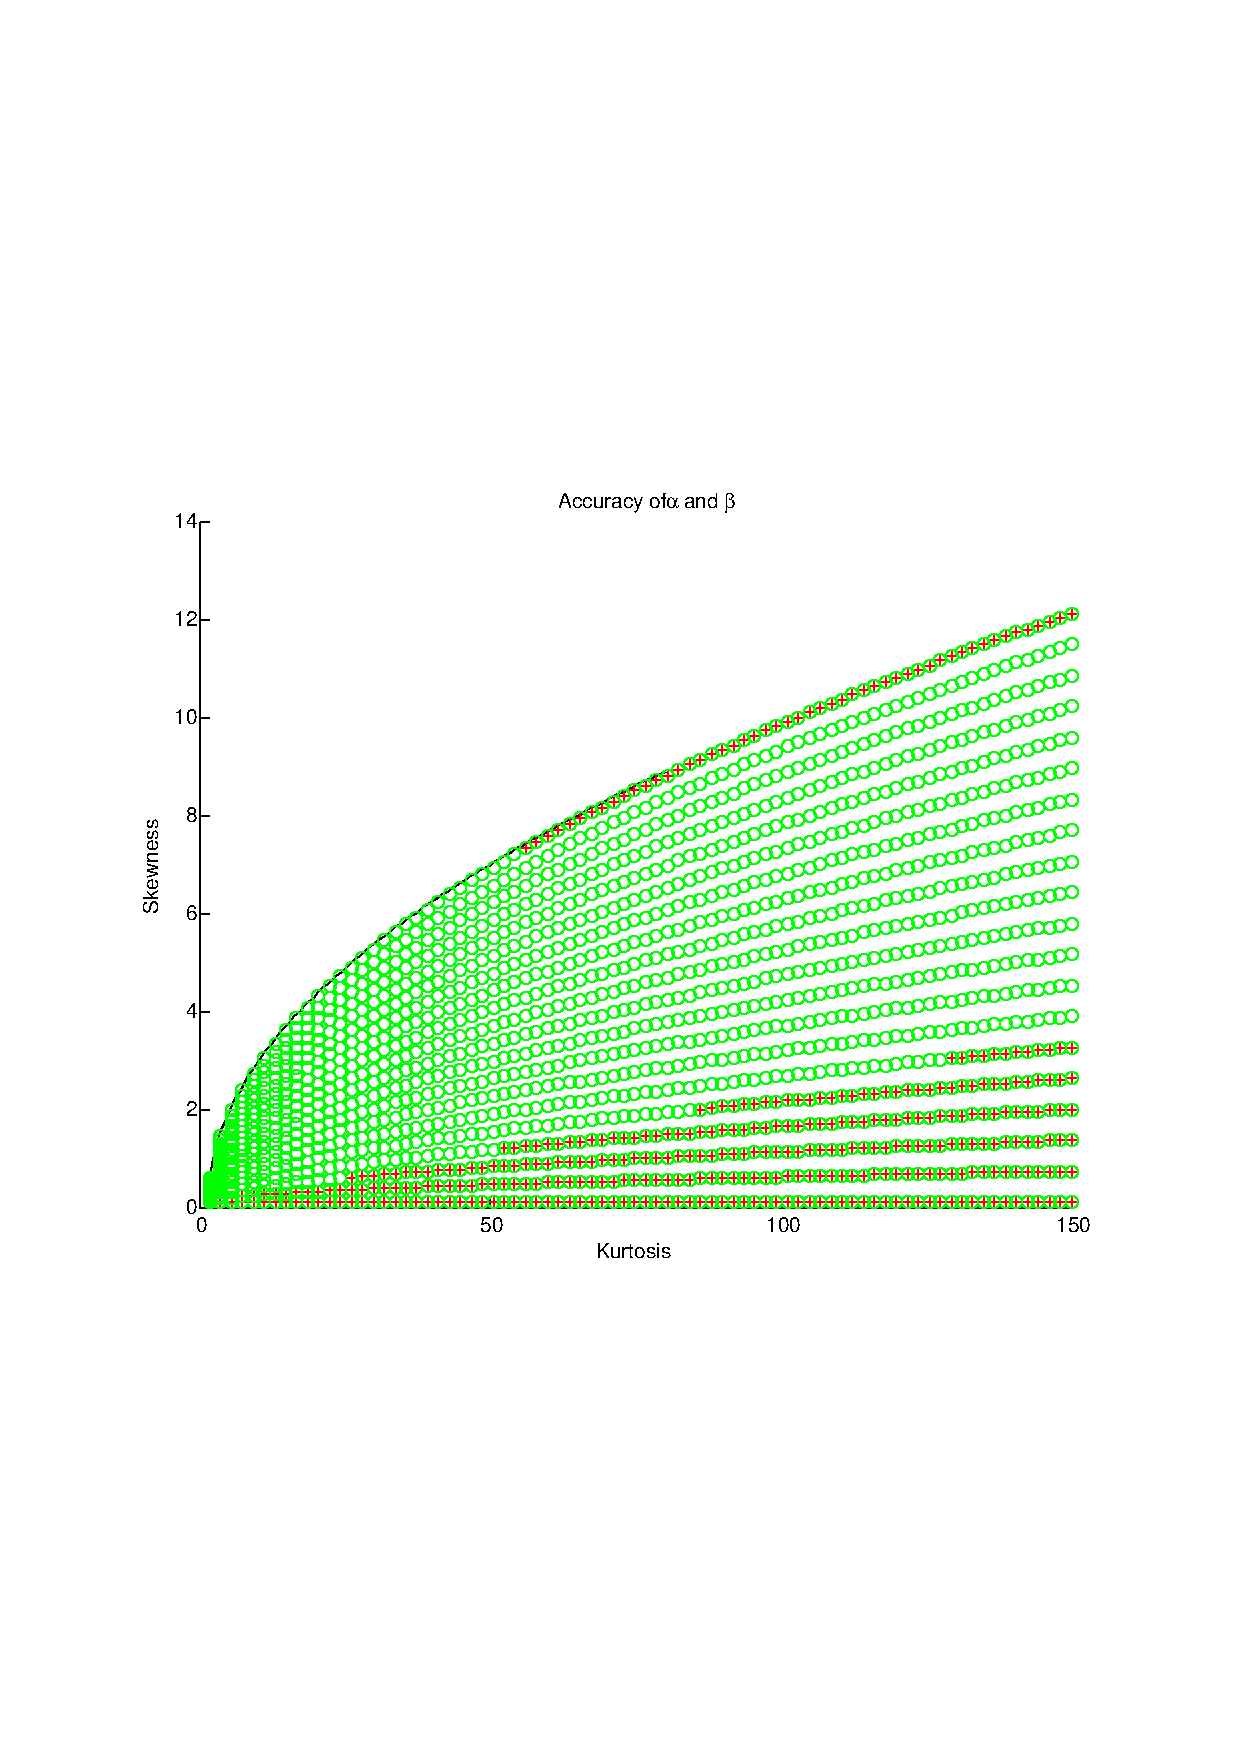
\includegraphics[trim= 1.5cm 7.5cm 1.cm 7.5cm,clip,scale=0.8
]{GautschiPrecisionHigh.pdf}
\caption{This figure represents the skewness-kurtosis domain for which a density exists (the domain is symmetric with respect to the horizontal axis). The circles represent those points for which we computed the parameters $\alpha$ and $\beta$. The symbol $+$ represents those points for which the distance between the original skewness and kurtosis and the recomputed skewness and kurtosis (after evaluation of the $\alpha$ and $\beta$) is larger than $10^{-5}$.}
\label{Fig_Domain}
\end{center}
\end{figure}
%% ----------------------------------------------------------------
\end{document}  % The End
%% ----------------------------------------------------------------